\documentclass[11pt]{beamer}
\usepackage[utf8]{inputenc}
\usepackage[T1]{fontenc}
\usepackage{lmodern}
\usepackage{amssymb}
\usepackage{pgfplots}
\usepackage{graphicx}
\usepackage{movie15}
\usepackage[french]{babel}
\usepackage{hyperref}
\usepackage{listings}

\usetheme{PaloAlto}

\addtobeamertemplate{footline}{\centering \insertframenumber/\inserttotalframenumber}

\begin{document}
	
\author[J.Delaeter C.Ghyselinck]{Joseph \bsc{Delaeter} et Corentin \bsc{Ghyselinck}}
\title{Projet Openxum}
\subtitle{Présentation orale 1}
\logo{
\includegraphics[width=45pt]{images/logo.jpg}}
\titlegraphic{
\includegraphics[width=50pt]{images/logo.jpg}}

  \begin{frame}
  \maketitle
  \end{frame}

  \begin{frame}
	\frametitle{Plan du cours}
	\tableofcontents
	\end{frame}
\section[Introduction]{Introduction}
  \begin{frame}
  \frametitle{Introduction}
  
  blablabla
  \end{frame}
\section[Description Jeux]{Descriptions Jeux} 

\subsection[Neutreeko]{Neutreeko} 

\begin{frame}

\frametitle{Neutreeko}
\subtitle{Neutreeko}
\begin{columns}[t]
\begin{column}{3cm}
	\begin{block}{Plateau}
	\centering 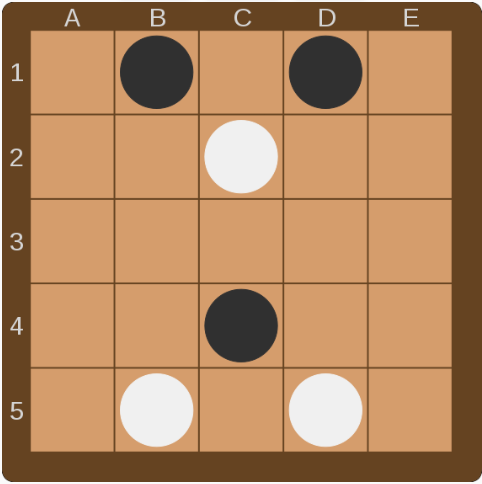
\includegraphics[width=50pt]{images/neut.png}
	\\
	\centering 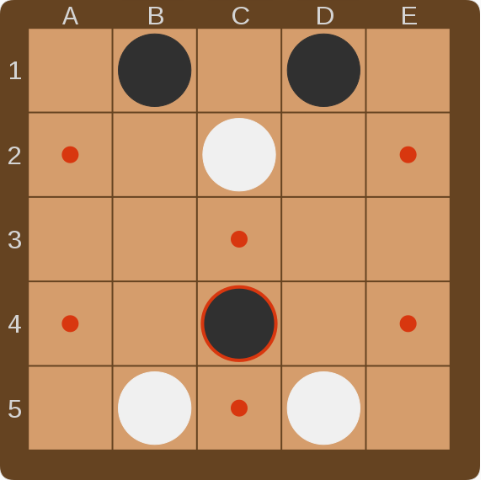
\includegraphics[width=50pt]{images/neut2.png}
	\\
	\centering 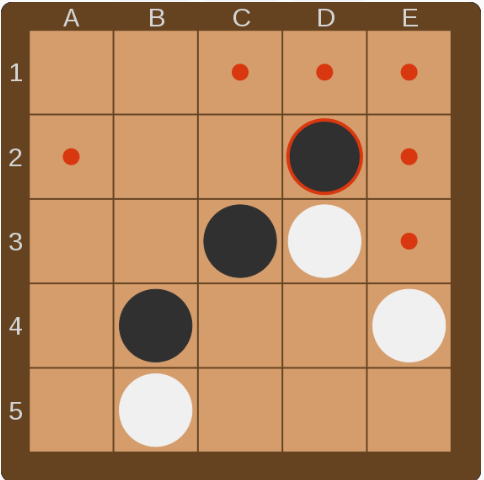
\includegraphics[width=50pt]{images/neut3.png}
	\end{block} 
\end{column}

\begin{column}{7cm}
	\begin{block}{Regle}
		\begin{itemize}
			\item La couleur Noire commence. 
			\item Une pièce se déplace dans toutes les directions.
			\item Un pion s'arrête si il rencontre un autre pion ou le bord du plateau.
			\item ni prise ni saut.
			\item Le but aligner ses trois pièces en continu.
		\end{itemize}
	\end{block}   
\end{column}
\end{columns}  
\end{frame}
  \subsection[Hnefatafl]{Hnefatafl}
\begin{frame}

\frametitle{Hnefatafl}
\subtitle{Hnefatafl}
\begin{columns}[t]
\begin{column}{4cm}
	\begin{block}{Plateau}
	\centering 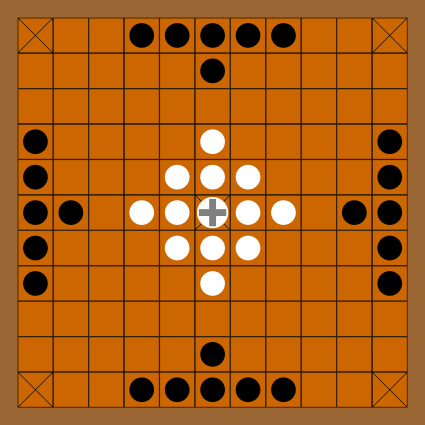
\includegraphics[width=75pt]{images/tafel.png}
	\begin{enumerate}
		\item \centering 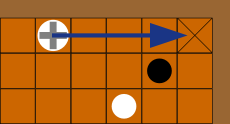
\includegraphics[width=60pt]{images/roi2.png}\\
		\item \centering 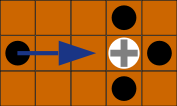
\includegraphics[width=60pt]{images/roi1.png}
	\end{enumerate}
	\end{block} 
\end{column}

\begin{column}{6cm}
	\begin{alertblock}{But du jeu}
		\begin{enumerate}
			\item joueur blanc:Amener le roi dans une forteresse .
			\item joueur noir:Prendre le roi adverse grâce à un encerclement du roi.
		\end{enumerate}
	\end{alertblock}   
\end{column}
\end{columns}  
\end{frame}

\begin{frame}

\frametitle{Hnefatafl}
\subtitle{Hnefatafl}
\begin{columns}[t]
\begin{column}{3cm}
	\begin{block}{Situation}
	\begin{enumerate}
		\item \centering 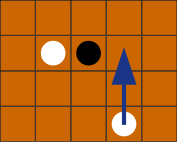
\includegraphics[width=50pt]{images/cap1.png}
		\item \centering 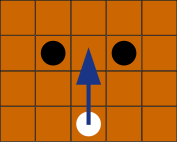
\includegraphics[width=50pt]{images/cap4.png}
		\item \centering 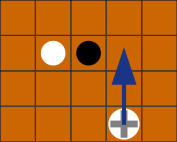
\includegraphics[width=50pt]{images/cap2.png}
		\\
		 \centering 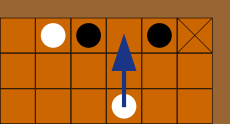
\includegraphics[width=50pt]{images/cap3.png}
	\end{enumerate}	
	\end{block} 
\end{column}

\begin{column}{7cm}
	\begin{block}{Condition d'élimination d'une piece adverse}
		\begin{enumerate}
		\item prise en tenaille d'un pion adverse
		\item prise en tenaille entre le roi et un pion adverse
		\item prise en tenaille par un adversaire et une forteresse. 
		\end{enumerate}
	\end{block}  
	
	\begin{alertblock}{Exception}
Un deplacement entre deux pions adverses n'élimine pas le pion.
	\end{alertblock}  
\end{column}
\end{columns}  
\end{frame}

\subsection[Kamisado]{Kamisado}
\begin{frame}
\frametitle{Kamisado}

\begin{center}
    \begin{block}{Plateau}
\centering 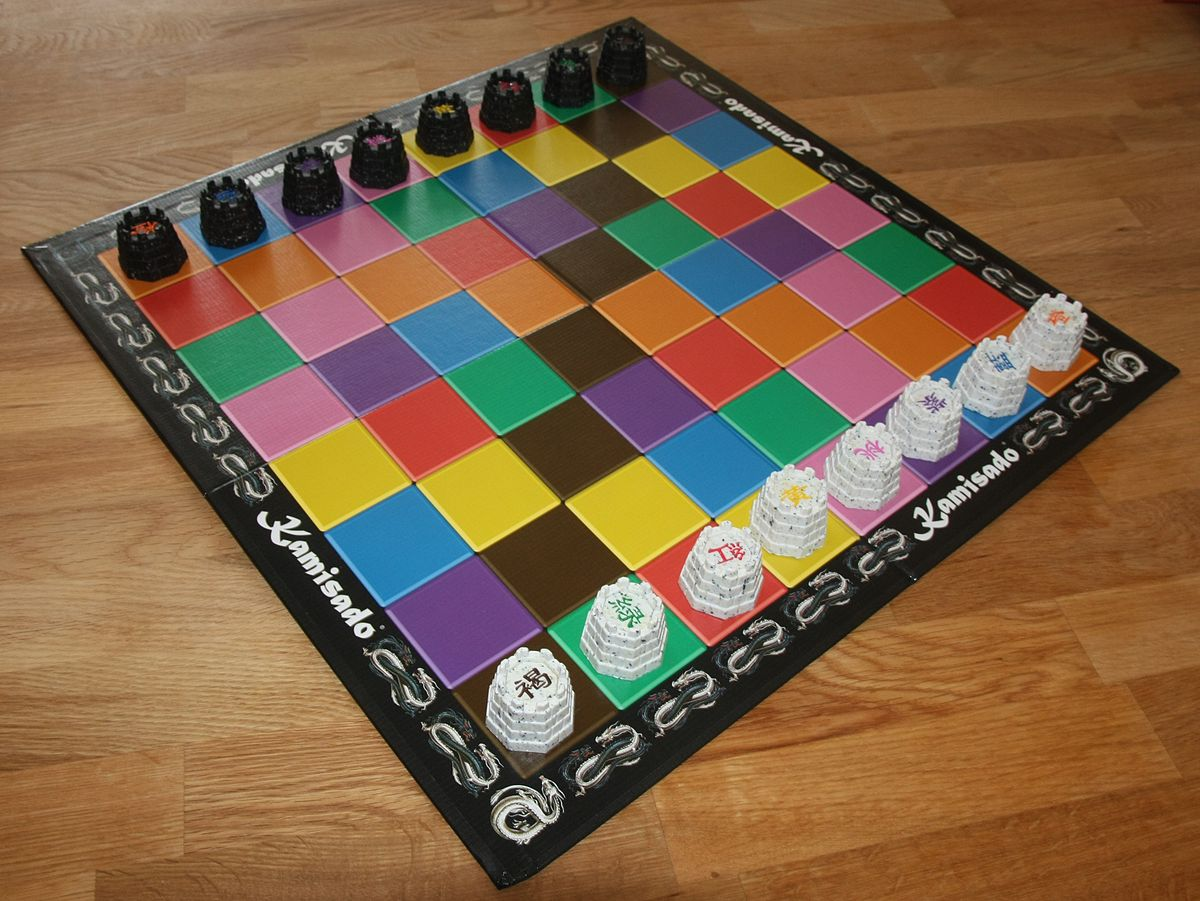
\includegraphics[width=200pt]{images/kami.jpg}
    \end{block}
\end{center}


\end{frame}

\begin{frame}
\color{blue}

\begin{columns}[t]
    \begin{column}{3cm}
        \begin{block}{Modes de jeu}
            \begin{itemize}
                \item Tour unique
                \item Standard
                \item Long
                \item Marathon
            \end{itemize}
        \end{block}
    \end{column}
    
    \begin{column}{7cm}
        \begin{block}{ Autres règles}
            \begin{itemize}
                \item Obligation de jouer
                \item Sinon le joueur passe son tour
                \item Impossible de passer à travers les pions, sauf en diagonale
                
                \item Si impossibilité de jouer, le dernier joueur à avoir jouer perd
            \end{itemize}
        \end{block}
    \end{column}
\end{columns}

\end{frame}
\subsection[Dakapo]{Dakapo}
\begin{frame}
\frametitle{Dakapo}
\subtitle{Dakapo}
\begin{columns}[t]
    \begin{column}{3cm}
        \begin{block}{Plateau}
            \centering 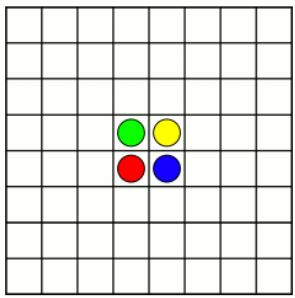
\includegraphics[width=80pt]{images/daka.JPG}
        \end{block}
    \end{column}
    
    \begin{column}{7cm}
        \begin{block}{Règles}
            \begin{itemize}
                \item Le premier joueur joue une couleur
                \item Un joueur ne peut pas jouer la couleur qui vient d'être jouer
                \item Les joueurs sont obligé de jouer sur une case adjacente à une case déjà occupée
                \item deux pièces de la même couleur ne peuvent pas être adjacente
                
                
            \end{itemize}
        \end{block}
    \end{column}
\end{columns}

\end{frame}

\section{Pourquoi ces jeux?}  
  \begin{frame}
  \frametitle{Pourquoi ces 4 jeux?}

\begin{block}{ titre du block }
      Texte, équations, image, tableau etc ...
\end{block}

\begin{block}{ titre du block }
      Texte, équations, image, tableau etc ...
\end{block}

\begin{block}{ titre du block }
      Texte, équations, image, tableau etc ...
\end{block}
			
  \end{frame}
    
\section{IA}
\subsection{Alpha Beta Elagage} 
  \begin{frame}
  \frametitle{Algorithme min-max}
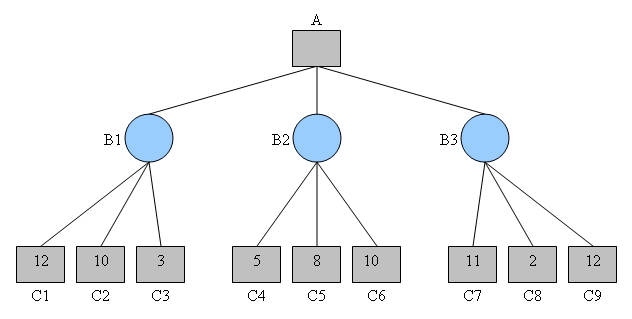
\includegraphics[width=150pt]{images/minmax.png}
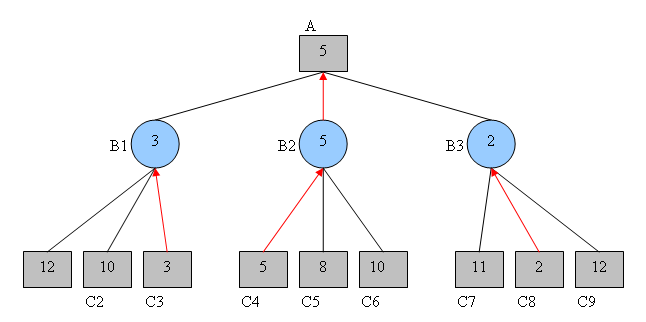
\includegraphics[width=150pt]{images/minmax2.png}
  \end{frame}
  \begin{frame}
  \frametitle{Elagage Alpha-Beta}
\centering 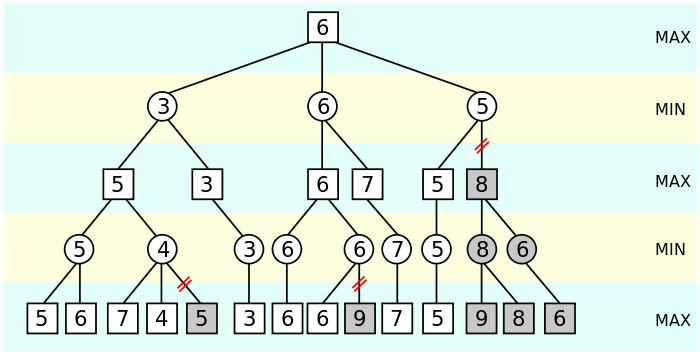
\includegraphics[width=150pt]{images/alphabeta.png}
\begin{block}{Interet de l'élagage}
            \begin{itemize}
                \item  réduire le nombre de nœuds évalués par MinMax
                \item augmentation de la profondeur de l'arbre à puissance de calcul équivalent
            \end{itemize}
\end{block}

\begin{alertblock}{But de l'élagage}
            \begin{itemize}
                \item Déplacement effectué de meilleur qualité
            \end{itemize}
\end{alertblock}



  \end{frame}  
  
 \subsection{MCTS}
 \begin{frame}
 \frametitle{MCTS}
 %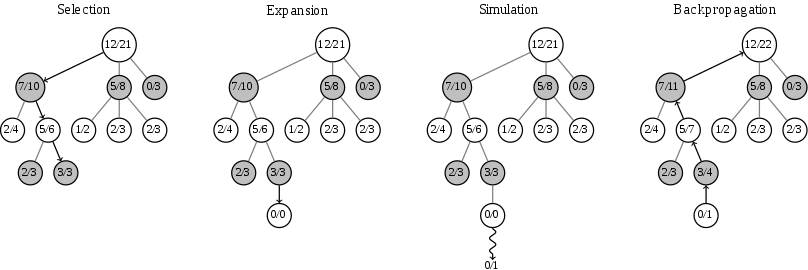
\includegraphics[width=340pt]{images/mcts.png}
 \color{blue}
 \vspace{1cm}
 
 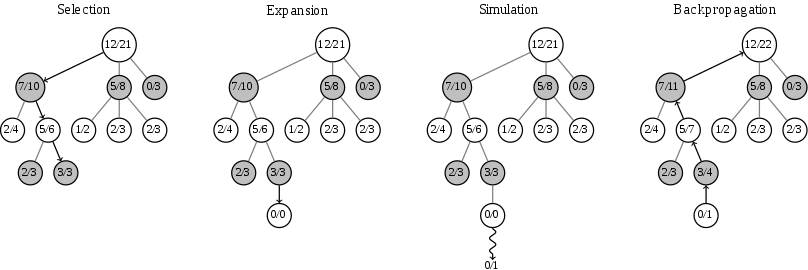
\includegraphics[width=280pt]{images/mcts.png}
 \vspace{0.5cm}
 \begin{itemize}
 	\item Sélection (Exploitation - Exploration)
 	\item Si  état non final -> Expansion
 	\item Simulation
 	\item Backpropagation : Maj score
 \end{itemize}
\end{frame}
\begin{frame}
\frametitle{MCTS}
Avantages
\begin{itemize}
\item généralité
\item calibrage
\end{itemize}
Limites
\begin{itemize}
\item      coûteux
\item non adapté aux jeux avec grand espace de recherche
\item améliorations potentiellement non efficace
\end{itemize}

\end{frame}
\section{Conclusion}
\begin{frame}
\frametitle{conclusion}
blablabla
\end{frame}

\end{document}